In this work, quantum algorithms based on Trotter schemes have been discussed and implemented on real quantum devices. Results from previous work \cite{BellUniversalCartan} have been rediscovered and used for time simulation of anisotropic Heisenberg Hamiltonians. Also, pulse efficient transpilation, following methods in \cite{RXZPulseEfficient}, has been implemented for the same purpose. Simulation results suggest that the best technique for simulating spin chains on real quantum devices is cross resonance pulse scaling. It has been shown that the main leverage of this method with respect to basis efficient transpilation is the reduced execution time of the control sequences on IBM Quantum devices. Since this method is quite hardware dependent, it is conjectured, though, that the basis efficient scheme discussed in this work might be a good alternative for simulating spin-1/2 Hamiltonians on CNOT-based quantum hardware. Since it has been shown by \cite{BellUniversalCartan} that this transpilation is optimal for two-qubit interaction, the transpilation discussed in section \ref{subsubsec:BasisEfficientCircuit} may be optimal for the Trotterization scheme used, on this type of hardware. It has also been shown that simulation of quantum systems using Trotterization requires balancing a tradeoff between trotter error and noise error due to decoherence. The integration time step $\Delta t$ must be chosen wisely so that the system evolves in the controlled error regime (fig. \ref{fig:FloquetDynamics}), but also the execution time of the algorithm is short enough to make efficient use of the finite coherence time of quantum devices. Although the algorithms seem to reproduce the physics of the system (for instance, expected value of observables) reasonably well for small times, faithful simulation of quantum systems using current devices seems to be impractical.

Although time simulation of quantum systems is impractical on current quantum devices, it has a wide range of applications to quantum computing. As a concluding remark, an application of quantum simulation to study ground state properties of Hamiltonians is discussed. For instance, the ground state energy of a quantum Hamiltonian may be computed using the adiabatic theorem \cite{Sakurai}. Consider time independent Hamiltonians $\hat{H}_0$ and $\hat{H}_m$, and an initial state $\ket{\psi_m}$ such that

\begin{equation}
    \hat{H}_m \ket{\psi_m} = \epsilon_m \ket{\psi_m},
    \label{eq:MixerGroundState}
\end{equation}

\noindent defined on a Hilbert space. Now, evolve a system in that initial state, under time-dependent Hamiltonian

\begin{equation}
    \hat{\mathcal{H}}(t) = \bigg(1-\frac{t}{T}\bigg)\hat{H}_m + \frac{t}{T}\hat{H}_0,
    \label{eq:AdiabaticHamiltonian}
\end{equation}

\noindent from $t=0$ to $t=T$. In the limit $T \rightarrow \infty$, the adiabatic theorem states that the final state of the system, $\ket{\psi}_0$, is such that 

\begin{equation}
    \hat{H}_0 \ket{\psi_0} = \epsilon_0 \ket{\psi_0},
    \label{eq:MixerGroundState}
\end{equation}

That is, the final state is a corresponding eigenstate of $\hat{H}_0$. In particular, if the initial state \ref{eq:MixerGroundState} is a ground state of the Hamiltonian $\hat{H}_m$, the final state is also a ground state of the Hamiltonian $\hat{H}_0$. By choosing a particularly simple Hamiltonian $\hat{H}_m$, whose ground state is easy to prepare on a quantum device, this type of evolution can be used to compute the ground state of a non trivial Hamiltonian. As an illustration, ground state energy of the three-qubit Hamiltonian

\begin{equation}
    \hat{H}_0 = \frac{1}{2}\sum_{i=0}^{1} \bigg(\hat{X}_i\hat{X}_{i+1} + 2\hat{Y}_i\hat{Y}_{i+1} + \frac{1}{2}\hat{Z}_i\hat{Z}_{i+1}\bigg) + \sum_{i=0}^{2} \hat{Z}_i
    \label{eq:AnnihilationHamiltonian}
\end{equation}

\noindent is computed. In figure \ref{fig:AnnihilationProcess}, the expected value of $\hat{H}_0$ after evolution for $t=T$ is plotted as a function of $T$. However, as may be seen, the evolution needs to be quite slow for convergence. This prevents practical usage of this tool on current quantum devices as seen in the present work.

\begin{figure}
    \centering
    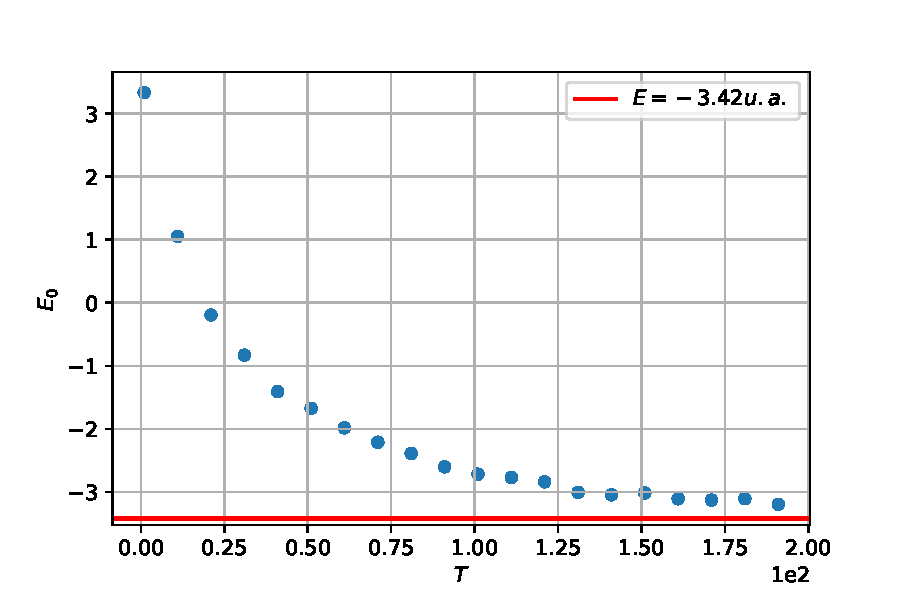
\includegraphics[scale=0.8]{AnnihilationDemo.pdf}
    \caption{Annihilation process for computing ground state energy of Hamiltonian \ref{eq:AnnihilationHamiltonian}. Exact ground state energy is represented by the solid red line. Data was generated using QASM simulator.}
    \label{fig:AnnihilationProcess}
\end{figure}

